\documentclass[11pt,a4paper]{article}

\usepackage[utf8]{inputenc}
\usepackage[T1]{fontenc}
\usepackage{mathpazo}
\usepackage[scaled=0.92]{helvet}
\usepackage[margin=1in]{geometry}
\usepackage{graphicx}
\usepackage{amsmath,amssymb,amsfonts}
\usepackage{booktabs}
\usepackage{tabularx}
\usepackage{setspace}
\usepackage{titlesec}
\usepackage{fancyhdr}
\usepackage{float}
\usepackage{caption}
\usepackage{microtype}
\usepackage{tikz}
\usepackage{xcolor}
\usepackage[hidelinks]{hyperref}

\usetikzlibrary{shapes.geometric, arrows.meta, positioning, calc, matrix, fit, backgrounds}

\setstretch{1.15}
\setlength{\parindent}{0pt}
\setlength{\parskip}{0.8em}
\sloppy

\titleformat{\section}{\normalfont\large\bfseries\sffamily}{\thesection}{1em}{}
\titleformat{\subsection}{\normalfont\normalsize\bfseries\sffamily}{\thesubsection}{1em}{}
\titleformat{\subsubsection}{\normalfont\normalsize\itshape\sffamily}{\thesubsubsection}{1em}{}

\pagestyle{fancy}
\fancyhf{}
\fancyhead[L]{\small\sffamily Requirement Engineering}
\fancyhead[R]{\small\sffamily\thepage}
\renewcommand{\headrulewidth}{0.4pt}

\captionsetup{font=small,labelfont=bf,labelsep=period}

\renewenvironment{abstract}
{\small
	\begin{center}\textbf{\sffamily Abstrak}\end{center}
	\begin{quote}}
	{\end{quote}}

\lstdefinestyle{code}{
	basicstyle=\ttfamily\small,
	frame=single,
	rulecolor=\color{black},
	breaklines=true,
	showstringspaces=false,
	columns=fullflexible,
	keepspaces=true,
	framesep=6pt,
	aboveskip=1em,
	belowskip=1em,
	xleftmargin=0pt
}

\lstdefinestyle{out}{
	basicstyle=\ttfamily\small,
	frame=tb,
	rulecolor=\color{black},
	breaklines=true,
	showstringspaces=false,
	columns=fullflexible,
	keepspaces=true,
	framesep=4pt,
	aboveskip=1em,
	belowskip=1em
}

\title{\vspace{-1.5cm}\textbf{\sffamily\LARGE Requirement Engineering\\ Panduan Praktis untuk Minggu Pertama}}
\author{
	\textbf{Muhammad Riduwan Khafidi} \\
	\small Program Studi Teknik Rekayasa Perangkat Lunak \\
	\small Politeknik Negeri Batam \\
	\small \texttt{4342611034@students.polibatam.ac.id}
}
\date{\small\today}

\begin{document}

\maketitle
\thispagestyle{empty}

\begin{abstract}
	Makalah ini adalah panduan praktis untuk minggu pertama mata kuliah Analisis dan Spesifikasi Kebutuhan Perangkat Lunak. Ia menjelaskan apa itu requirement engineering, mengapa ia penting, masalah umum yang muncul bila diabaikan, serta dua proses requirement yang lazim dipakai di industri. Tujuh visualisasi dan tiga tabel menyertai penjelasan agar konsep abstrak menjadi konkret. Sebuah studi kasus berisi sepuluh langkah menunjukkan artefak yang harus dihasilkan pada setiap tahap. Lembar rujukan cepat di akhir merangkum istilah yang wajib dikuasai sebelum pertemuan berikutnya.
\end{abstract}

\section{Pendahuluan}

\subsection{Analogi Pembuka}

Bayangkan seorang tukang bangunan yang hendak mendirikan rumah. Ia tidak mulai dengan memasang batu bata. Ia duduk bersama pemilik rumah dulu: berapa kamar, di mana dapur, apakah perlu garasi, berapa anggarannya. Percakapan itu bukan gambar rumah. Tapi tanpa percakapan itu, tukang akan membangun kamar mandi di ruang tamu.

Requirement engineering adalah percakapan itu. Ia adalah seni menggali apa yang sebenarnya diinginkan pemilik rumah sebelum satu batu pun diletakkan.

\subsection{Mengapa Topik Ini Penting}

Perangkat lunak dibuat untuk memenuhi tujuan dan kebutuhan pengguna. Ia tidak boleh dibuat berdasarkan asumsi developer. Kesalahan yang ditemukan pada tahap requirement jauh lebih murah diperbaiki daripada kesalahan yang baru ditemukan setelah sistem diluncurkan. Inilah sebabnya requirement engineering diletakkan di awal seluruh siklus pengembangan.

\subsection{Peta Pembahasan}

Makalah ini disusun sebagai berikut. Bagian kedua menjelaskan apa itu requirement dan level-levelnya. Bagian ketiga menjelaskan mengapa ia penting dengan kurva biaya perubahan. Bagian keempat memetakan enam masalah umum. Bagian kelima membedakan product requirement dan project requirement. Bagian keenam membedah aktivitas requirement engineering. Bagian ketujuh membandingkan proses Volere dan Agile. Bagian kedelapan menyajikan studi kasus sepuluh langkah. Bagian kesembilan sampai kesebelas merangkum kesalahan umum, lembar rujukan cepat, serta tiga prinsip penutup.

\section{Apa Itu Requirement}

Requirement adalah spesifikasi tentang apa yang harus diimplementasikan. Ia mendeskripsikan bagaimana sistem harus berperilaku, properti atau atribut apa yang harus dimiliki, dan batasan apa yang membatasi proses pengembangannya. Requirement mencakup dua perspektif sekaligus: perspektif pengguna tentang perilaku sistem, dan perspektif developer tentang karakteristik internal sistem.

Perhatikan Gambar~\ref{fig:anatomy-req}. Sebuah requirement yang baik menyentuh empat lapis: perilaku, properti, atribut, dan batasan.

\begin{figure}[H]
	\centering
	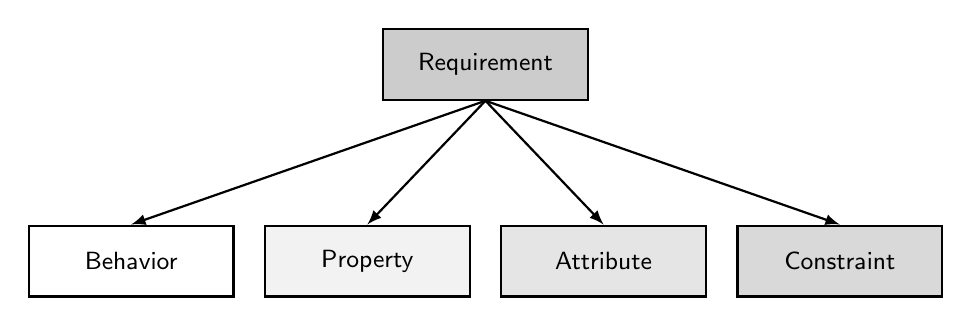
\begin{tikzpicture}[
			box/.style={rectangle, draw=black, thick, minimum width=2.6cm, minimum height=0.9cm, align=center, font=\sffamily\small},
			line/.style={draw, thick, -latex}
		]
		\node[box, fill=black!20] (req) at (0, 0) {Requirement};

		\node[box, fill=white]    (beh)  at (-4.5, -2.5) {Behavior};
		\node[box, fill=black!5]  (prop) at (-1.5, -2.5) {Property};
		\node[box, fill=black!10] (attr) at ( 1.5, -2.5) {Attribute};
		\node[box, fill=black!15] (cons) at ( 4.5, -2.5) {Constraint};

		\draw[line] (req.south) -- (beh.north);
		\draw[line] (req.south) -- (prop.north);
		\draw[line] (req.south) -- (attr.north);
		\draw[line] (req.south) -- (cons.north);
	\end{tikzpicture}
	\caption{Anatomi requirement yang terdiri dari empat lapis.}
	\label{fig:anatomy-req}
\end{figure}

Contohnya, pada sistem pemesanan tiket kereta: perilaku adalah ``sistem menampilkan jadwal kereta berdasarkan tanggal yang dipilih''; properti adalah ``sistem menyimpan riwayat pemesanan selama tiga tahun''; atribut adalah ``halaman jadwal memuat paling banyak dua puluh baris per halaman''; dan batasan adalah ``sistem harus mematuhi UU Perlindungan Data Pribadi''.

Requirement juga hidup di beberapa level. Perhatikan Gambar~\ref{fig:req-levels}. Di level paling atas ada business requirement yang berbicara tentang tujuan sponsor. Di tengah ada user requirement yang berbicara tentang tugas pengguna. Di bawah ada system requirement yang dipecah menjadi fungsional dan non-fungsional. Semakin ke bawah, semakin detail dan semakin teknis.

\begin{figure}[H]
	\centering
	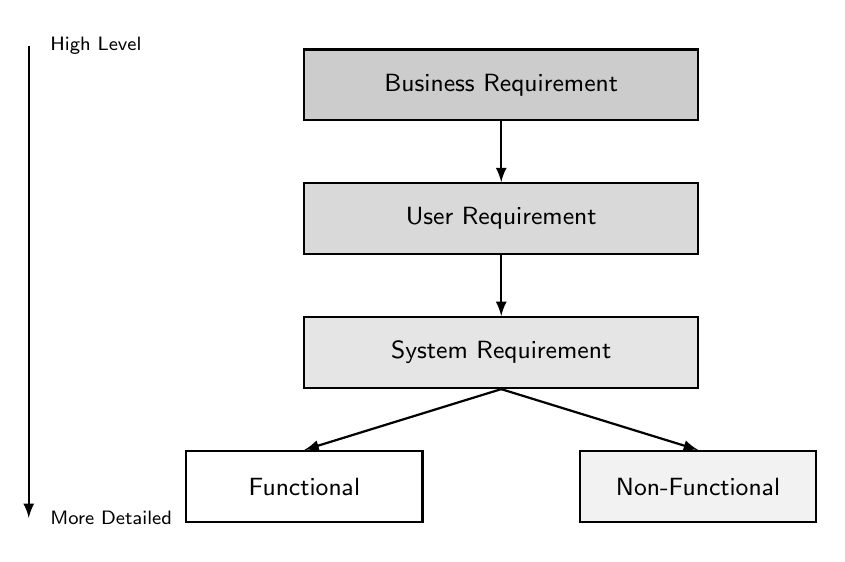
\begin{tikzpicture}[
			box/.style={rectangle, draw=black, thick, minimum width=5cm, minimum height=0.9cm, align=center, font=\sffamily\small},
			leaf/.style={rectangle, draw=black, thick, minimum width=3cm, minimum height=0.9cm, align=center, font=\sffamily\small},
			line/.style={draw, thick, -latex},
			note/.style={font=\sffamily\scriptsize, align=center}
		]
		\node[box, fill=black!20] (biz)  at (0,  5.0) {Business Requirement};
		\node[box, fill=black!15] (user) at (0,  3.3) {User Requirement};
		\node[box, fill=black!10] (sys)  at (0,  1.6) {System Requirement};

		\node[leaf, fill=white]   (fun) at (-2.5, -0.1) {Functional};
		\node[leaf, fill=black!5] (nfr) at ( 2.5, -0.1) {Non-Functional};

		\draw[line] (biz.south)  -- (user.north);
		\draw[line] (user.south) -- (sys.north);
		\draw[line] (sys.south)  -- (fun.north);
		\draw[line] (sys.south)  -- (nfr.north);

		\draw[line] (-6, 5.5) -- (-6, -0.5);
		\node[note, anchor=west] at (-5.85, 5.5) {High Level};
		\node[note, anchor=west] at (-5.85, -0.5) {More Detailed};
	\end{tikzpicture}
	\caption{Hierarki level requirement dari high level menuju detail.}
	\label{fig:req-levels}
\end{figure}

Pemetaan level ini penting karena requirement yang hanya menyebut perilaku, tanpa menyebut properti, atribut, dan batasan, hampir pasti akan menghasilkan perdebatan di tengah pengembangan. Ia juga menjelaskan mengapa requirement yang ditulis dengan bahasa sponsor berbeda dari requirement yang ditulis dengan bahasa developer.

\section{Mengapa Requirement Engineering Penting}

Aturan industri: semakin awal masalah ditemukan, semakin murah biaya memperbaikinya. Perhatikan Gambar~\ref{fig:cost-curve}. Biaya perubahan naik perlahan di tahap requirement, lalu melonjak tajam di tahap produksi.

\begin{figure}[H]
	\centering
	\begin{tikzpicture}[
			axis/.style={draw, thick, -latex},
			curve/.style={draw, thick, smooth},
			lbl/.style={font=\scriptsize\sffamily},
			point/.style={circle, fill=black, inner sep=2pt}
		]
		\draw[axis] (0,0) -- (11,0) node[right, font=\small\sffamily] {Waktu};
		\draw[axis] (0,0) -- (0,5) node[above, font=\small\sffamily] {Biaya};

		\draw[curve] (0.5, 0.3) .. controls (2.5, 0.45) and (4.0, 0.9) .. (6.5, 2.2) .. controls (8.0, 3.1) and (9.0, 4.2) .. (10.0, 4.85);

		\node[point] at (0.5, 0.3)  {};
		\node[point] at (2.5, 0.5)  {};
		\node[point] at (4.5, 1.05) {};
		\node[point] at (6.5, 2.2)  {};
		\node[point] at (9.0, 4.15) {};

		\node[lbl, below] at (0.5, -0.15) {Req};
		\node[lbl, below] at (2.5, -0.15) {Design};
		\node[lbl, below] at (4.5, -0.15) {Coding};
		\node[lbl, below] at (6.5, -0.15) {Testing};
		\node[lbl, below] at (9.0, -0.15) {Produksi};
	\end{tikzpicture}
	\caption{Kurva biaya perubahan sepanjang siklus proyek.}
	\label{fig:cost-curve}
\end{figure}

Mengubah kode sumber pada sistem yang sudah diluncurkan jauh lebih sulit dan berisiko daripada mengubah desain sistem di tahap awal. Karena itu, setiap jam yang diinvestasikan untuk menggali requirement di awal akan menghemat puluhan jam di akhir.

\section{Masalah Umum pada Proyek Perangkat Lunak}

Enam masalah berikut adalah yang paling sering muncul. Perhatikan Gambar~\ref{fig:problems}.

\begin{figure}[H]
	\centering
	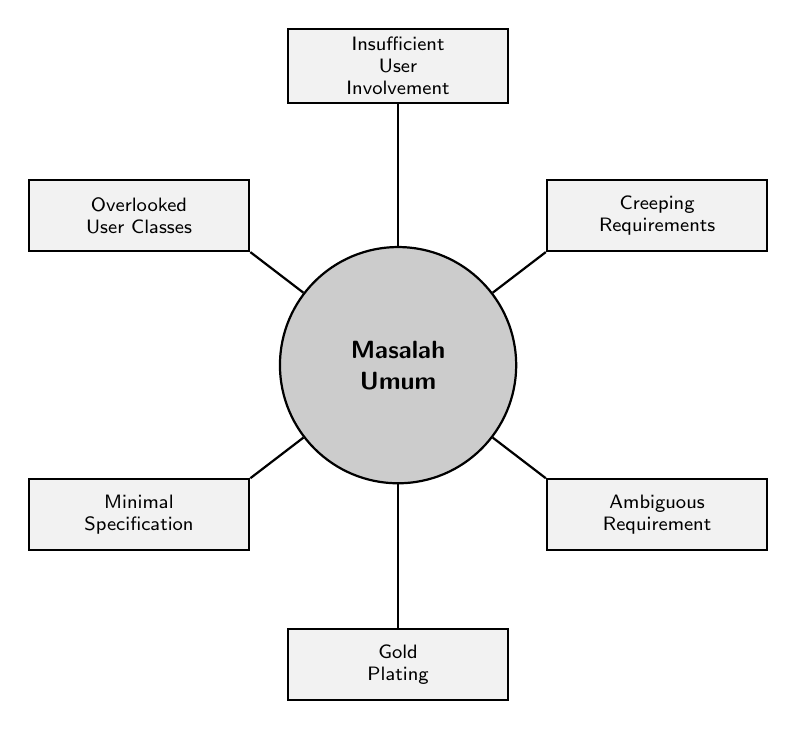
\begin{tikzpicture}[
			prob/.style={rectangle, draw=black, thick, fill=black!5, minimum width=2.8cm, minimum height=0.9cm, align=center, font=\sffamily\scriptsize, inner sep=3pt},
			center/.style={circle, draw=black, thick, fill=black!20, minimum size=3cm, align=center, font=\sffamily\small\bfseries},
			line/.style={draw, thick}
		]
		\node[center] (c) at (0,0) {Masalah\\Umum};

		\node[prob] (p1) at (0,     3.8) {Insufficient\\User\\Involvement};
		\node[prob] (p2) at (3.29,  1.9) {Creeping\\Requirements};
		\node[prob] (p3) at (3.29, -1.9) {Ambiguous\\Requirement};
		\node[prob] (p4) at (0,    -3.8) {Gold\\Plating};
		\node[prob] (p5) at (-3.29,-1.9) {Minimal\\Specification};
		\node[prob] (p6) at (-3.29, 1.9) {Overlooked\\User Classes};

		\draw[line] (c) -- (p1.south);
		\draw[line] (c) -- (p2.south west);
		\draw[line] (c) -- (p3.north west);
		\draw[line] (c) -- (p4.north);
		\draw[line] (c) -- (p5.north east);
		\draw[line] (c) -- (p6.south east);
	\end{tikzpicture}
	\caption{Enam masalah umum dalam proyek perangkat lunak.}
	\label{fig:problems}
\end{figure}

\textbf{Pertama, insufficient user involvement.} Kurangnya keterlibatan pengguna mengakibatkan miskomunikasi, yang pada akhirnya menunda jadwal proyek.

\textbf{Kedua, creeping user requirements.} Klien terus menambah dan mengubah requirement bahkan setelah pengembangan dimulai, tanpa memahami kompleksitas dan dampaknya.

\textbf{Ketiga, ambiguous requirement.} Requirement yang ambigu membuat tiap pihak punya tafsir berbeda, sehingga developer bisa membangun solusi untuk masalah yang salah.

\textbf{Keempat, gold plating.} Developer menambahkan fitur ekstra yang tidak diminta, dengan asumsi pengguna akan memakainya. Jika ternyata tidak, seluruh usaha itu terbuang.

\textbf{Kelima, minimal specification dan perencanaan tidak akurat.} Spesifikasi minim memicu banyak perubahan di tengah jalan, dan perencanaan yang tidak akurat menyebabkan estimasi anggaran dan jadwal meleset.

\textbf{Keenam, overlooked user classes.} Satu produk biasanya dipakai berbagai kelas pengguna. Jika ada kelas yang terlupakan, kebutuhan mereka tidak akan terpenuhi.

\section{Product Requirement dan Project Requirement}

Dua istilah ini sering tertukar. Perhatikan Gambar~\ref{fig:prod-vs-proj}.

\begin{figure}[H]
	\centering
	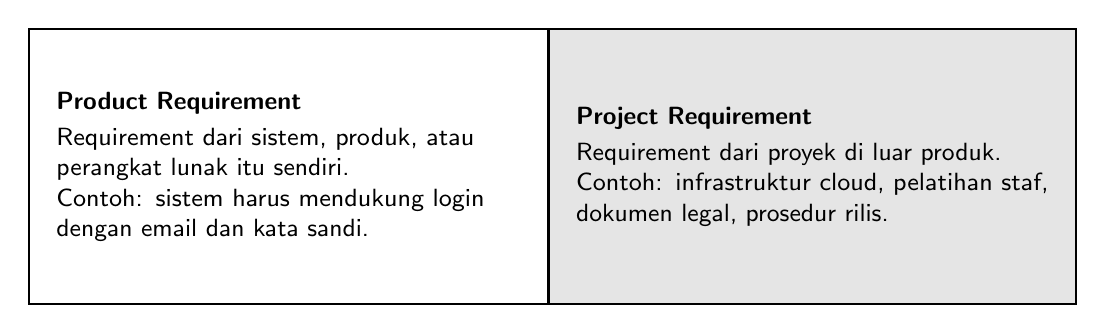
\begin{tikzpicture}[
			box/.style={rectangle, draw=black, thick, text width=6cm, align=left, font=\sffamily\small, inner sep=10pt, minimum height=3.5cm}
		]
		\node[box, fill=white, anchor=north west] (a) at (-6.3, 0) {
			\textbf{Product Requirement} \\[2pt]
			Requirement dari sistem, produk, atau perangkat lunak itu sendiri. \\
			Contoh: sistem harus mendukung login dengan email dan kata sandi.
		};
		\node[box, fill=black!10, anchor=north west] (b) at (0.3, 0) {
			\textbf{Project Requirement} \\[2pt]
			Requirement dari proyek di luar produk. \\
			Contoh: infrastruktur cloud, pelatihan staf, dokumen legal, prosedur rilis.
		};
	\end{tikzpicture}
	\caption{Perbedaan product requirement dan project requirement.}
	\label{fig:prod-vs-proj}
\end{figure}

\textbf{Product requirement} berbicara tentang software-nya: fitur apa, alur apa, batasan apa. \textbf{Project requirement} berbicara tentang proyek yang mengembangkan software itu: sumber daya, infrastruktur, pelatihan, legal, dan prosedur rilis. Seorang analis requirement wajib bisa membedakan keduanya, karena solusi untuk masing-masing ada di ranah yang berbeda.

\section{Aktivitas Requirement Engineering}

Requirement engineering terdiri dari dua aktivitas besar. Perhatikan Gambar~\ref{fig:re-activities}.

\begin{figure}[H]
	\centering
	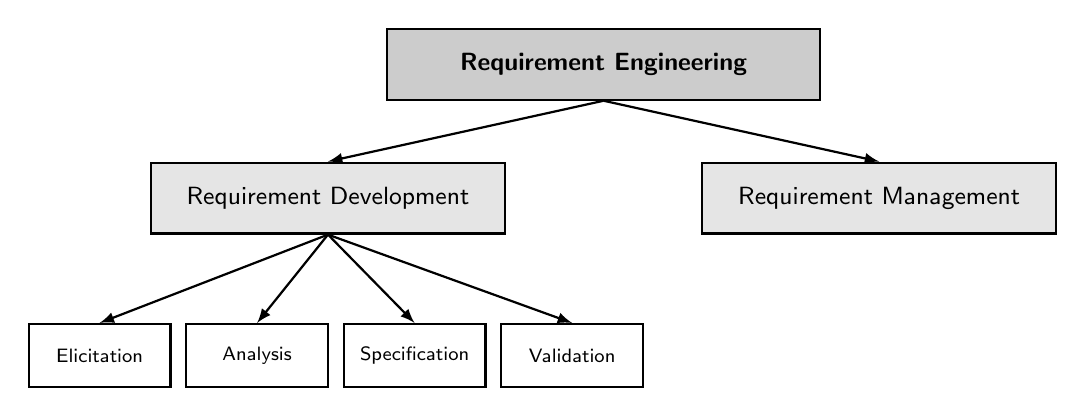
\begin{tikzpicture}[
			root/.style={rectangle, draw=black, thick, fill=black!20, minimum width=5.5cm, minimum height=0.9cm, align=center, font=\sffamily\small\bfseries},
			mid/.style={rectangle, draw=black, thick, fill=black!10, minimum width=4.5cm, minimum height=0.9cm, align=center, font=\sffamily\small},
			leaf/.style={rectangle, draw=black, thick, fill=white, minimum width=1.8cm, minimum height=0.8cm, align=center, font=\sffamily\scriptsize},
			line/.style={draw, thick, -latex}
		]
		\node[root] (eng) at (0, 5) {Requirement Engineering};
		\node[mid]  (dev) at (-3.5, 3.3) {Requirement Development};
		\node[mid]  (mgmt) at (3.5, 3.3) {Requirement Management};

		\node[leaf] (e) at (-6.4, 1.3) {Elicitation};
		\node[leaf] (a) at (-4.4, 1.3) {Analysis};
		\node[leaf] (s) at (-2.4, 1.3) {Specification};
		\node[leaf] (v) at (-0.4, 1.3) {Validation};

		\draw[line] (eng.south) -- (dev.north);
		\draw[line] (eng.south) -- (mgmt.north);
		\draw[line] (dev.south) -- (e.north);
		\draw[line] (dev.south) -- (a.north);
		\draw[line] (dev.south) -- (s.north);
		\draw[line] (dev.south) -- (v.north);
	\end{tikzpicture}
	\caption{Aktivitas requirement engineering dan pembagiannya.}
	\label{fig:re-activities}
\end{figure}

\textbf{Requirement Development} mencakup seluruh aktivitas yang berhubungan dengan eksplorasi, evaluasi, dokumentasi, dan konfirmasi requirement. Ia terdiri dari empat sub-aktivitas: elicitation (menggali), analysis (menganalisis), specification (menuliskan), dan validation (memvalidasi).

\textbf{Requirement Management} mencakup aktivitas menjaga rencana proyek tetap selaras dengan requirement, melacak status dan perubahan requirement sepanjang proyek, serta meninjau usulan perubahan dan mengevaluasi dampaknya sebelum disetujui.

Perbedaan keduanya sederhana. Development menjawab pertanyaan \textit{apa kebutuhannya}. Management menjawab pertanyaan \textit{bagaimana perubahannya dikendalikan}.

\section{Dua Proses Requirement yang Lazim}

Di industri, ada dua pendekatan besar. Perhatikan Gambar~\ref{fig:volere-vs-agile}.

\begin{figure}[H]
	\centering
	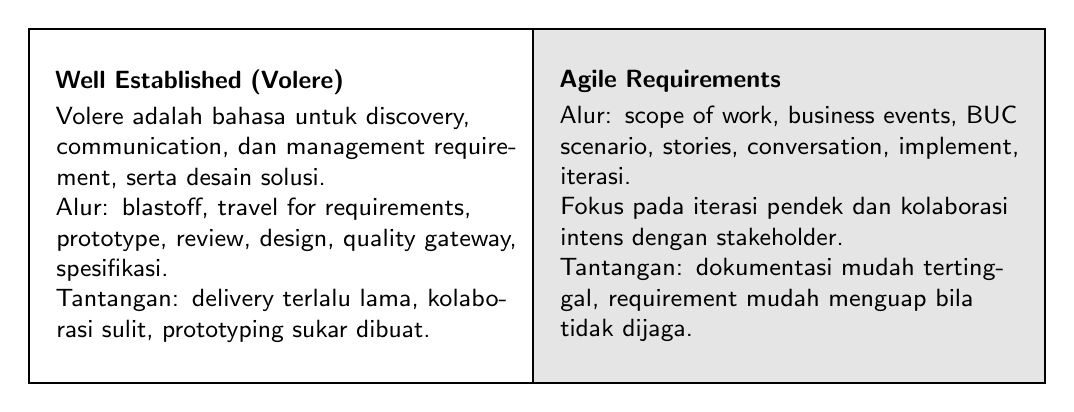
\begin{tikzpicture}[
			box/.style={rectangle, draw=black, thick, text width=5.8cm, align=left, font=\sffamily\small, inner sep=10pt, minimum height=4.5cm}
		]
		\node[box, fill=white, anchor=north west] (a) at (-6.1, 0) {
			\textbf{Well Established (Volere)} \\[2pt]
			Volere adalah bahasa untuk discovery, communication, dan management requirement, serta desain solusi. \\
			Alur: blastoff, travel for requirements, prototype, review, design, quality gateway, spesifikasi. \\
			Tantangan: delivery terlalu lama, kolaborasi sulit, prototyping sukar dibuat.
		};
		\node[box, fill=black!10, anchor=north west] (b) at (0.3, 0) {
			\textbf{Agile Requirements} \\[2pt]
			Alur: scope of work, business events, BUC scenario, stories, conversation, implement, iterasi. \\
			Fokus pada iterasi pendek dan kolaborasi intens dengan stakeholder. \\
			Tantangan: dokumentasi mudah tertinggal, requirement mudah menguap bila tidak dijaga.
		};
	\end{tikzpicture}
	\caption{Perbandingan proses requirement Volere dan Agile.}
	\label{fig:volere-vs-agile}
\end{figure}

Volere cocok untuk proyek dengan requirement yang relatif stabil dan tim yang tersebar. Agile cocok untuk proyek yang requirement-nya cepat berubah dan tim berkumpul di satu tempat. Tidak ada yang lebih unggul secara mutlak. Yang penting adalah memilih satu, dan konsisten.

\section{Perbandingan Ringkasan}

Tabel~\ref{tab:summary} merangkum perbedaan kunci antar konsep yang telah dibahas.

\begin{table}[H]
	\centering
	\caption{Ringkasan konsep utama minggu pertama.}
	\label{tab:summary}
	\footnotesize
	\begin{tabularx}{\textwidth}{l X X}
		\toprule
		Aspek             & Konsep Pertama                   & Konsep Kedua                                \\
		\midrule
		Jenis requirement & Product requirement              & Project requirement                         \\
		Aktivitas RE      & Requirement development          & Requirement management                      \\
		Sub-aktivitas dev & Elicitation, analysis            & Specification, validation                   \\
		Fokus aktivitas   & Menggali dan mendokumentasikan   & Mengendalikan perubahan                     \\
		Proses industri   & Volere (terstruktur)             & Agile (iteratif)                            \\
		Tantangan         & Delivery lama, prototyping sukar & Dokumentasi tertinggal, requirement menguap \\
		\bottomrule
	\end{tabularx}
\end{table}

\section{Studi Kasus: Sepuluh Langkah yang Harus Kamu Hasilkan}

Bagian ini memandu langkah demi langkah untuk memproduksi deliverable minggu pertama. Contoh kasus: Sistem Informasi Perpustakaan Kampus. Setiap langkah menghasilkan satu artefak yang bisa dikumpulkan.

\subsection{Langkah 1: Baca Kasus dan Identifikasi Masalah}

Sebelum menulis apa pun, baca deskripsi kasus sampai habis. Tulis satu paragraf masalah dalam bahasa sehari-hari.

\begin{lstlisting}[style=out]
		Masalah:
		Proses peminjaman buku di perpustakaan kampus masih
		manual. Mahasiswa mengisi formulir kertas, pustakawan
		memeriksa satu per satu, dan pengembalian sering
		terlambat tanpa pemberitahuan. Akibatnya antrean
		panjang di jam sibuk dan denda tidak konsisten.
	\end{lstlisting}

\subsection{Langkah 2: Daftar Stakeholder}

Tulis siapa saja yang akan terpengaruh keputusan proyek.

\begin{lstlisting}[style=out]
		Stakeholder:
		1. Kepala Perpustakaan (project sponsor)
		2. Pustakawan (end user aktif)
		3. Mahasiswa (end user pasif)
		4. Dosen (peminjam jangka panjang)
		5. Tim IT kampus (pengelola infrastruktur)
	\end{lstlisting}

\subsection{Langkah 3: Daftar User Class}

Kelompokkan pengguna berdasarkan frekuensi, kemampuan, dan hak akses.

\begin{lstlisting}[style=out]
		User Class:
		1. Pustakawan (favored) - memakai tiap hari
		2. Mahasiswa - memakai tiap minggu
		3. Dosen - memakai tiap bulan
		4. Kepala Perpustakaan - memakai untuk laporan
	\end{lstlisting}

\subsection{Langkah 4: Tulis Business Requirement}

Jelaskan mengapa proyek ini ada.

\begin{lstlisting}[style=out]
		Business Requirement:
		Mengotomasi proses peminjaman dan pengembalian buku
		agar antrean di jam sibuk berkurang, denda terhitung
		konsisten, dan kepala perpustakaan mendapat laporan
		bulanan tanpa harus menghitung manual.
	\end{lstlisting}

\subsection{Langkah 5: Tulis Vision Statement}

Rumuskan arah produk dalam satu kalimat.

\begin{lstlisting}[style=out]
		Vision Statement:
		Sistem Informasi Perpustakaan adalah aplikasi berbasis
		web yang memungkinkan mahasiswa meminjam buku tanpa
		antre, pustakawan mengelola stok dengan cepat, dan
		kepala perpustakaan memantau peminjaman secara
		real-time.
	\end{lstlisting}

\subsection{Langkah 6: Tentukan Scope}

Pisahkan apa yang masuk dan apa yang tidak masuk.

\begin{lstlisting}[style=out]
		In Scope:
		- Pencarian katalog buku
		- Peminjaman dan pengembalian
		- Perhitungan denda otomatis
		- Laporan bulanan

		Out of Scope:
		- Rekomendasi buku berbasis AI
		- Pembayaran denda via payment gateway
		- Aplikasi mobile native
	\end{lstlisting}

\subsection{Langkah 7: Tulis User Story}

Gunakan format role-goal-benefit.

\begin{lstlisting}[style=out]
		User Story US-01:
		Sebagai mahasiswa,
		saya ingin mencari buku berdasarkan judul atau penulis,
		agar saya tidak perlu berkeliling rak.

		User Story US-02:
		Sebagai pustakawan,
		saya ingin memindai kartu mahasiswa untuk peminjaman,
		agar proses pinjam selesai di bawah satu menit.
	\end{lstlisting}

\subsection{Langkah 8: Tulis Functional Requirement}

Rumuskan perilaku sistem dengan input dan output.

\begin{lstlisting}[style=out]
		FR-01: Sistem menampilkan daftar buku yang cocok
		dengan kata kunci pencarian.
		Input: kata kunci (string), maksimal 50 karakter.
		Output: daftar maksimal 20 baris berisi judul,
		penulis, dan status ketersediaan.

		FR-02: Sistem mencatat peminjaman saat pustakawan
		memindai kartu mahasiswa.
		Input: nomor kartu (string), kode buku (string).
		Output: transaksi peminjaman dengan tanggal jatuh tempo
		14 hari setelah tanggal pinjam.
	\end{lstlisting}

\subsection{Langkah 9: Tulis Non-Functional Requirement}

Rumuskan kualitas sistem.

\begin{lstlisting}[style=out]
		NFR-01 (Performance): Pencarian katalog selesai dalam
		waktu kurang dari 2 detik untuk 10.000 judul.

		NFR-02 (Availability): Sistem tersedia 99,5 persen
		waktu dalam satu bulan, di luar jadwal pemeliharaan.

		NFR-03 (Security): Password pengguna disimpan dengan
		hash bcrypt. Sesi berakhir setelah 30 menit idle.
	\end{lstlisting}

\subsection{Langkah 10: Validasi dan Kelola}

Periksa apakah semua requirement konsisten, lalu tetapkan proses perubahan.

\begin{lstlisting}[style=out]
		Checklist Validasi:
		- Semua stakeholder sudah membaca dan setuju
		- Tidak ada requirement yang saling bertentangan
		- Setiap requirement bisa diuji (testable)
		- Setiap perubahan setelah ini harus melalui
		change request dengan persetujuan project sponsor
	\end{lstlisting}

Sepuluh langkah di atas menghasilkan tiga artefak siap kumpul: dokumen vision and scope, dokumen requirement, dan matriks validasi. Inilah yang dimaksud dengan deliverable minggu pertama.

\section{Kesalahan Umum}

Tabel~\ref{tab:mistakes} merangkum kesalahan yang paling sering muncul saat mengerjakan tugas minggu pertama.

\begin{table}[H]
	\centering
	\caption{Kesalahan umum pada pekerjaan requirement minggu pertama.}
	\label{tab:mistakes}
	\footnotesize
	\begin{tabularx}{\textwidth}{l X X}
		\toprule
		Kesalahan                                             & Akibat                               & Perbaikan                                                     \\
		\midrule
		Menulis solusi, bukan requirement                     & Dokumen jadi desain, bukan kebutuhan & Tulis apa yang dibutuhkan, bukan bagaimana mewujudkannya      \\
		Mencampur product dan project requirement             & Scope melebar tak terkendali         & Pisahkan dua daftar dan beri label jelas                      \\
		Melewatkan satu user class                            & Kebutuhan kelas itu tidak terpenuhi  & Periksa ulang daftar stakeholder sebelum menutup dokumen      \\
		Requirement ambigu seperti ``cepat'' tanpa angka      & Developer menebak-nebak              & Ganti dengan angka terukur: ``kurang dari 2 detik''           \\
		Menulis requirement yang tidak bisa diuji             & Validasi tidak bisa dilakukan        & Ubah jadi kalimat dengan input, proses, dan output yang jelas \\
		Scope tidak pernah ditulis eksplisit                  & Fitur baru terus masuk tanpa kendali & Selalu cantumkan in scope dan out of scope                    \\
		Menganggap elicitation selesai setelah satu wawancara & Kebutuhan tidak lengkap              & Lakukan minimal tiga sumber: wawancara, observasi, dokumen    \\
		Lupa menetapkan proses perubahan                      & Requirement berubah tanpa jejak      & Tetapkan change request dan persetujuan sponsor               \\
		\bottomrule
	\end{tabularx}
\end{table}

Dua kesalahan yang paling sering muncul adalah \textbf{mencampur solusi dengan requirement} dan \textbf{tidak menulis scope secara eksplisit}. Keduanya sama-sama berakar pada satu hal: ketergesaan. Sempatkan satu putaran penuh untuk membaca ulang sebelum menyerahkan.

\section{Lembar Rujukan Cepat}

Tabel~\ref{tab:cheat} adalah ringkasan istilah dan artefak yang wajib dikuasai sebelum pertemuan kedua.

\begin{table}[H]
	\centering
	\caption{Lembar rujukan cepat untuk minggu pertama.}
	\label{tab:cheat}
	\footnotesize
	\begin{tabularx}{\textwidth}{l X}
		\toprule
		Kebutuhan atau Istilah     & Definisi atau Artefak                                                         \\
		\midrule
		Requirement                & Spesifikasi apa yang harus diimplementasikan oleh sistem                      \\
		Requirement engineering    & Disiplin menggali, menganalisis, mendokumentasikan, dan memvalidasi kebutuhan \\
		Stakeholder                & Siapa pun yang terpengaruh aktivitas dan keputusan proyek                     \\
		User class                 & Kelompok pengguna berdasarkan frekuensi, kemampuan, dan hak akses             \\
		Product champion           & Perwakilan user class yang menjadi jembatan ke analis                         \\
		Business requirement       & Alasan mengapa proyek dilakukan, biasanya di level sponsor                    \\
		User requirement           & Tugas yang bisa dilakukan pengguna dengan produk                              \\
		System requirement         & Requirement di level sistem: fungsional dan non-fungsional                    \\
		Functional requirement     & Perilaku yang harus dilakukan sistem                                          \\
		Non-functional requirement & Kualitas yang harus dimiliki sistem                                           \\
		Product requirement        & Requirement dari sistem/produk/software                                       \\
		Project requirement        & Requirement dari proyek di luar produk                                        \\
		Requirement development    & Elicitation, analysis, specification, validation                              \\
		Requirement management     & Tracking status, change control, impact evaluation                            \\
		Elicitation                & Aktivitas menggali kebutuhan dari stakeholder                                 \\
		Vision                     & Arah jangka panjang produk                                                    \\
		Scope                      & Bagian yang dikerjakan pada rilis atau iterasi saat ini                       \\
		Volere                     & Proses requirement terstruktur untuk discovery hingga design                  \\
		Agile requirements         & Proses requirement iteratif berbasis cerita pengguna                          \\
		\bottomrule
	\end{tabularx}
\end{table}

\section{Kesimpulan}

Requirement engineering adalah fondasi seluruh siklus pengembangan perangkat lunak. Ia terdiri dari dua aktivitas besar, yaitu requirement development dan requirement management, dengan empat sub-aktivitas pengembangan: elicitation, analysis, specification, dan validation. Tiga prinsip penutup:

\begin{enumerate}
	\item \textbf{Gali dulu, jangan menebak.} Perangkat lunak tidak boleh dibangun berdasarkan asumsi developer. Setiap requirement wajib punya jejak ke stakeholder nyata.
	\item \textbf{Pisahkan produk dari proyek.} Product requirement dan project requirement harus ditulis sebagai dua daftar terpisah agar scope tidak melebar tanpa kendali.
	\item \textbf{Uji sebelum menyerahkan.} Requirement yang tidak bisa diuji bukan requirement, melainkan harapan. Ubah setiap kalimat menjadi sesuatu yang bisa diverifikasi dengan input, proses, dan output yang jelas.
\end{enumerate}

Pada pertemuan berikutnya, prinsip-prinsip ini akan dipakai untuk mempelajari stakeholder dan aktivitas requirement engineering secara lebih mendalam. Lembar rujukan cepat di atas adalah bekal minimum yang harus dibawa.

\newpage
\section*{Referensi}
\addcontentsline{toc}{section}{Referensi}

\begin{thebibliography}{99}

	\bibitem{sommerville}
	Sommerville, I. (2016).
	\textit{Software Engineering} (10th ed.).
	Pearson.

	\bibitem{wiegers}
	Wiegers, K., \& Beatty, J. (2013).
	\textit{Software Requirements} (3rd ed.).
	Microsoft Press.

	\bibitem{robertson}
	Robertson, S., \& Robertson, J. (2012).
	\textit{Mastering the Requirements Process: Getting Requirements Right} (3rd ed.).
	Addison-Wesley.

	\bibitem{iiba}
	International Institute of Business Analysis. (2015).
	\textit{A Guide to the Business Analysis Body of Knowledge (BABOK Guide)} (v3.0).
	IIBA.

	\bibitem{pressman}
	Pressman, R. S., \& Maxim, B. R. (2020).
	\textit{Software Engineering: A Practitioner's Approach} (9th ed.).
	McGraw-Hill Education.

	\bibitem{ieee830}
	IEEE. (1998).
	\textit{IEEE Recommended Practice for Software Requirements Specifications (IEEE Std 830-1998)}.
	Institute of Electrical and Electronics Engineers.

\end{thebibliography}

\end{document}
